% !TEX root = ../SinkhornDivergenceUnbalanced.tex

\section{Numerical illustrations}
\label{sec:numerical}

\subsection{A synthetic example with gradient flows}
We now present numerical examples and applications of our results based on the algorithm of Section~\ref{sec-implementation}. Our implementation of the functionals and the code needed to reproduce the experiments below is available at:\\
\centerline{\url{https://github.com/thibsej/unbalanced-ot-functionals}.}


We present numerical experiments on gradient flows.
Given a set of particles $\theta = \{(x_i, r_i)_i \}$ with coordinates $x_i \in\R^d$ and masses $r_i \in\R_+$, one wishes to study their trajectories under a potential $\theta\mapsto F(\theta)$.
The particles intialized at $t=0$ by $\theta_0$ undergo the dynamic $\partial_t\theta(t) = - \nabla F(\theta(t))$.
Such flows have been extensively studied for Partial Differential Equations.
They also gained attention in machine learning to study convergence of neural networks~\cite{chizat2018global}.
%As discussed in the introduction, these flows have been studied extensively in the field of . 
%They also gained attention in the machine learning community, allowing researcher to shed some light on the convergence of overparameterized one-layer neural networks~\cite{chizat2018global}.

We consider the same setting as~\cite{chizat2019sparse}.
We consider a target measure $\be\in\Mmp(\R^d)$ and the potential $\al\mapsto\Sb(\al,\be)$, as one would do in e.g. generative learning in imaging~\cite{arjovsky2017wasserstein}.
The measure $\al$ represents the model we train, parameterized as $\al_\theta = \sum_i^n  r_i^2 \de_{x_i}$ with parameter $\theta = ((x_i, r_i))_i\in(\R^2\times\R_+)^n$.
Minimizing $\Sb(\cdot,\be)$ amounts to run the following gradient steps
%
\begin{align*}
	x_i^{(t+1)} & = x_i^{(t)} - \eta_x \nabla_{x_i} \Sb(\al_\theta^{(t)}, \be),                  \\
	r_i^{(t+1)} & = r_i^{(t)}.\exp\big( - 2\eta_x \nabla_{r_i} \Sb(\al_\theta^{(t)}, \be) \big),
\end{align*}
where $(\eta_x, \eta_r)>0$ are two learning steps.
%
The update on $r_i$ is called a mirror descent step, and is used to enforce that $r_i\geq 0$.
We retrieve the exact gradient flow when $(\eta_x, \eta_r)\rightarrow 0$.
Using such model $\al_\theta$ and such updates is proved in~\cite{chizat2019sparse} to be equivalent to a gradient flow in the space $\Mmp(\Xx)$, in contrast with classical flows optimizing over $\Mmp_1(\Xx)$.


%We discretize the measure $\al$ with a set of weighted particles and run a gradient flow with respect to them. 
%In optimisation terms, this amounts to parameterizing $\al_\theta$ using a sum of weighted diracs and running gradient descent with respect to the parameters of the particles $\theta = \{(x_i, r_i)_i \}$. 
%Following~\cite{chizat2019sparse}, we use a different parameterization of the measure $\al_\theta=\sum_i^n  r_i^2 \de_{x_i}$ as a measure $\sum_i \de_{(x_i, r_i)}$ on the cone $(\R^d\times\R_+)^n$ equipped with the local metric
%\begin{align*}
%  \dotp{(x_1,r_1)}{(x_2,r_2)}_{(x,r)} = \frac{\eta_x}{r^2}\dotp{x_1}{x_2}_x + \eta_r r_1 r_2.
%\end{align*}
%
% We use forward gradient steps with respect to the positions and mirror descent steps with respect to the mass. Using such model makes the optimization on the cone equivalent to optimizing the energy $\Sb(.,\be)$ on the space of positive measures. 
%
%Given two learning rates $(\eta_x, \eta_r)$, the updates on the parameters read at time $t$ for any $i$ (see~\cite[Algorithm 1]{chizat2019sparse})


We run the experiments in several settings.
Wa always take the Euclidean distance $\C(x,y)=\norm{x-y}^2_2$ on the unit square $[0,1]^2$, constant learning rates $(\eta_x, \eta_r) = (60, 0.3)$, a radius $\sqrt{\rho}=\sqrt{10^{-1}}$, and a default blur radius of $\sqrt{\epsilon}=\sqrt{10^{-3}}$.
In each timeframe we display iterations $[5, 10, 20, 50, 300]$ of the gradient descent steps.
Each dot represents a particle, and the diameter represents its mass.

Figures~\ref{fig-flow-reg} (rows 1 and 2) show the difference between using $\OTb$ and the (debiased) Sinkhorn divergence $\Sb$.
Note that for $\OTb$ (row 1) the model $\al_\theta$ concentrates (i.e. suffers the \emph{entropic bias}) while for $\Sb$ it approaches $\be$ up to details of size $\sqrt{\epsilon}$.
%
One the same figure, comparing rows 2 and 3 shows the influence of $\epsilon$, which operates a low pass smoothing.
If $\epsilon$ is chosen too large then $\al_\theta$ discards finer details.
%
Figure~\ref{fig-flow-tv} shows the impact of changing $\D_\phi$ on the mass variation dynamics.
For instance, one retrieves a partial transport behaviour for $\rho\TV$.


\newcommand{\myrot}[1]{ \rotatebox{90}{\small \hspace{2mm} #1}}

\newcommand{\myimg}[1]{\includegraphics[width=0.16\textwidth]{images/#1}}
\newcommand{\myimgRow}[1]{ % 
	\myimg{density_display-c} & %
	\myimg{#1_frame5-c} &  %
	\myimg{#1_frame10-c} & %
	\myimg{#1_frame20-c} & %
	\myimg{#1_frame50-c} & %
	\myimg{#1_frame300-c}   %
}
\newcommand{\myimgRowMod}[1]{ % 
	\myimg{density_display-c} & %
	\myimg{#1_frame5-c} &  %
	\myimg{#1_frame10-c} & %
	\myimg{#1_frame20-c} & %
	\myimg{#1_frame50-c} & %
	\myimg{#1_frame300-c.png}   %
}

\begin{figure}[p]
	\centering
	\if 0  %%% UNCOMMENT FOR HIGH RES %%%
		\begin{tabular}{@{}c@{\hspace{1mm}}c@{}c@{}c@{}c@{}c@{}c@{}c@{}}
			\myrot{$\OTb(\cdot,\be)$ } & \myrot{$\epsilon=10^{-6}$} & \myimgRow{flow_ot/regularized}                                                     \\
			\myrot{$\Sb(\cdot,\be)$}   & \myrot{$\epsilon=10^{-6}$} & \myimgRow{flow_kl/kl_neat}                                                         \\
			\myrot{$\Sb(\cdot,\be)$}   & \myrot{$\epsilon=10^{-2}$} & \myimgRow{flow_blur/kl_blur}                                                       \\
			                           &                            & $t=0$                          & $t=0.02$ & $t=0.03$ & $t=0.07$ & $t=0.17$ & $t=1$
		\end{tabular}
	\fi
	\includegraphics[width=\linewidth]{images/fig-flow-1}
	\caption{
		Comparison of gradient for of three different discrepancy when using $\D_\phi=\rho\KL$.
		%
		The target measure $\be$ is displayed in blue, while the evolving measure $\al_t$ is displayed using a rainbow color scheme that allows us to track individual particles.
	}
	\label{fig-flow-reg}
	%\end{figure}

	\vspace*{.5cm}

	%\begin{figure}
	%  \centering
	\if 0  %%% UNCOMMENT FOR HIGH RES %%%
		\begin{tabular}{@{}c@{}c@{}c@{}c@{}c@{}c@{}c@{}}
			\myrot{$\rho\TV$ }                 & \myimgRow{flow_tv/total_variation}                                                     \\
			\myrot{$\text{RG}_{[0.7,\, 1.3]}$} & \myimgRow{flow_range/range}                                                            \\
			\myrot{$\iota_{(=)}$}              & \myimgRow{flow_bal/balanced}                                                           \\
			                                   & $t=0$                              & $t=0.02$ & $t=0.03$ & $t=0.07$ & $t=0.17$ & $t=1$
		\end{tabular}
	\fi
	\includegraphics[width=\linewidth]{images/fig-flow-2}
	\caption{Flow of $\Sb(.,\be)$ with different type of divergence $\D_\phi$, from top to bottom: Total Variation (TV), range constraint and balanced OT. }
	\label{fig-flow-tv}
\end{figure}




\subsection{An application: 3D scene flow estimation}


The theory of unbalanced and entropy-regularized OT is motivated by
applications to noisy data. Our goal is to enable the use of transport-based tools
on problems that are a ``good but imperfect’’ fit
for the standard Monge--Kantorovitch model.

To make this point clear, we showcase the use of our robust OT tools on a real applied problem: the estimation of displacement vectors (``3D flow’’) between two views of the same 3D scene that have been acquired at times $t$ and $t+\Delta t$. This is a fundamental task in computer vision, with major applications to automated driving \cite{vedula1999three}.

As illustrated in Fig.~\ref{fig:kitti}, we consider two point clouds
$x_1$, \ldots, $x_\text{N}$ (``source frame’’) and
$y_1$, \dots, $y_\text{M}$ (``target frame’’) that have been acquired
by a binocular device or a LiDAR scanner.
For this experiment, we rely on a cropped scene from
the standard KITTI dataset \cite{kitti,flownet3d}.
We intend to estimate the positions
$p_1$, \dots, $p_\text{N}$ of all points $x_i$ at time $t+\Delta t$.
We stress that both 3D frames have
been sampled independently from each other,
which means that the Ground Truth results
$p_1^\text{GT}$, \dots, $p_\text{N}^\text{GT}$
that are provided in the dataset
are \emph{not} in perfect correspondence with
the target points $y_1$, \dots, $y_\text{M}$.


% \afterpage{\clearpage}
\begin{figure}[p]
	\centering
	\captionsetup{width=\linewidth}
	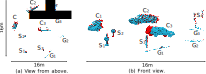
\includegraphics[width=\linewidth]{images/scene_flow/view.pdf}
	\caption{\textbf{3D scene extracted from the KITTI dataset \cite{kitti}.}
		The source (red) and target (blue) point clouds are sampled with
		4,000 points each: they are not in perfect correspondence with each other.
		In the coordinate system of the acquisition device,
		we observe 10 solid objects:
		3 cars in rigid motion ($\text{C}_1$, $\text{C}_2$, $\text{C}_3$);
		4 immobile traffic signs and poles ($\text{S}_1$, $\text{S}_2$, $\text{S}_3$, $\text{S}_4$);
		3 parts of the ground that have been correctly removed
		from the source frame in the pre-processing step but remain visible
		in the target frame ($\text{G}_1$, $\text{G}_2$, $\text{G}_3$).}
	\label{fig:kitti}

	\vspace*{.5cm}
	\vfill
	\includegraphics[width=\linewidth]{images/scene_flow/plans.pdf}
	\caption{\textbf{Estimation of the 3D scene flow} with different values for the
		blur ($\sqrt{\epsilon}$) and reach ($\sqrt{\rho}$) parameters.
		We focus on a detail of Fig.~\ref{fig:kitti}
		($\text{C}_3$, $\text{S}_4$, $\text{G}_2$, $\text{G}_3$)
		and display the registration result $p_1$, \dots, $p_\text{N}$
		with green points and green arrows that link them to the source points $x_i$.
	}
	\label{fig:plan}

	\vspace*{.5cm}
	\vfill
	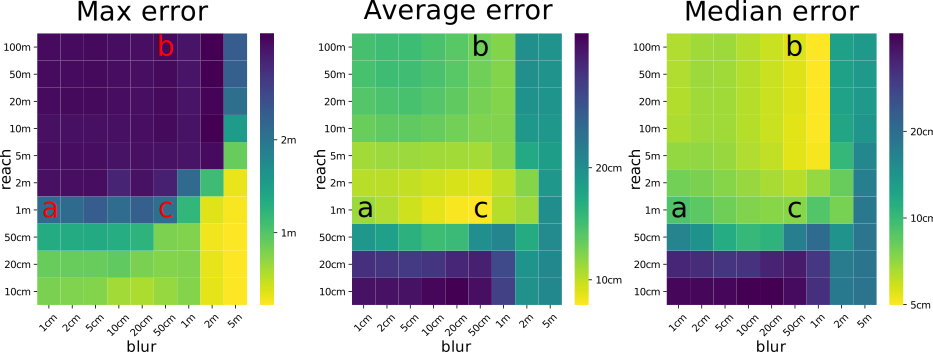
\includegraphics[width=\linewidth]{images/scene_flow/tables.pdf}
	\caption{\textbf{Quantitative evaluation.} We display the maximum, average and median
		3D error between the final registrations $p_i$
		and the ground truth target points $p_i$ for varying values of
		the blur ($\sqrt{\varepsilon}$) and reach ($\sqrt{\rho}$) parameters
		in Eq.~(\ref{eq:scene_flow_descent}).
		Letters ``a'', ``b'' and ``c'' correspond to the three visualizations
		of Fig.~\ref{fig:plan}.}
	\label{fig:kitti_tables}
\end{figure}

In the context of automated driving,
a pre-processing step (the ``segmentation'')
removes points that correspond to
the pavement on the ground.
As a consequence, we can understand the scene flow between any two
frames as a collection of small, independent and rigid transformations
of solid objects such as cars, trees and bikes.
OT theory is perfectly suited to this class of geometric
deformations, and recent progress on numerical solvers
have opened the door
to real-time processing for this data \cite{robot}.

To demonstrate the influence of entropic regularization
and of the softening of the marginal constraints
on the scene flow estimation, we study a descent-based algorithm
along the lines of the previous Section.
We work with a quadratic cost $\C(x,y)=\tfrac{1}{2}\norm{x-y}^2_2$
and a Kullback--Leibler penalty on the marginal constraints.
We initialize our flowing point cloud on the source frame
($x_i^{(0)} = x_i$) with uniform weights equal to $1/\text{N}$
and update the point positions with:

\begin{align}
	\forall\, i \in \llbracket 1, \text{N} \rrbracket, ~~
	x_i^{(t+1)} = x_i^{(t)} - \text{N}\, \nabla_{x_i^{(t)}} \Sb\big(\tfrac{1}{\text{N}} \textstyle\sum_{k=1}^\text{N} \delta_{x_k^{(t)}}, \tfrac{1}{\text{M}}\textstyle\sum_{k=1}^\text{M} \delta_{y_k} \big)~.
	\label{eq:scene_flow_descent}
\end{align}
The final registration corresponds to the point cloud
$p_1=x_1^{(10)}$, \dots, $p_\text{N}=x_\text{N}^{(10)}$
after 10 iterations.
The main parameters of our method are the blur ($\sqrt {\epsilon}$)
and reach ($\sqrt{\rho}$) scales for the Sinkhorn divergence $\Sb$,
which are both homogeneous to distances in 3D space.

In this experiment, we rely on the GeomLoss library \cite{feydy2018interpolating,feydy2020thesis} to evaluate
the debiased Sinkhorn divergence $\Sb$ and its gradient.
We keep the GeomLoss ``scaling'' parameter equal to 0.9
to ensure a high precision in the OT solver.
As detailed in \cite[Section 3.3]{feydy2020thesis},
this implementation relies on
symmetrized iterations and an annealing
heuristic to speed up computations
beyond the fully rigorous Algorithm~\ref{alg:sinkhorn}
that is presented in this paper.
We display registration results in Fig.~\ref{fig:plan}
and make the following observations:

\begin{itemize}
	\item Unbalanced OT corresponds to the limit case where the reach
	      parameter ($\sqrt{\rho}$) is finite and the blur parameter ($\sqrt
		      {\epsilon}$) is smaller than the typical distance between any two
	      samples. This setting is illustrated in Fig.~\ref{fig:plan}.a: on the one
	      hand, the registration is robust to the presence of segmentation
	      artifacts for the pavement in the target frame; but on the other hand,
	      the final registration ($p_i$, green) overfits to the target point cloud ($y_j$, blue).
	      The estimated scene flow is unrealistically non-smooth.

	\item Entropy-regularized OT corresponds to the limit case where the blur
	      parameter ($\sqrt{\epsilon}$) is significantly larger than zero and the
	      reach parameter ($\sqrt{\rho}$) is equal to $+\infty$ or is much larger
	      than the diameter of the 3D scene. As illustrated in Fig.~\ref{fig:plan}.b, the registration is smooth but is highly impacted by artifacts that are present
	      in the data: our method matches the front-end of the car to a part of the
	      pavement that was (erroneously) left visible in the target frame.

	\item Unbalanced, entropy-regularized OT is robust to both types of perturbations. As
	      illustrated in Fig.~\ref{fig:plan}.c, picking intermediate values
	      for both of the blur ($\sqrt{\epsilon}$) and reach ($\sqrt{\rho}$) parameters allows us to recover a smooth displacement field
	      that is not thrown in disarray by segmentation artifacts.

\end{itemize}

\noindent
We provide a quantitative analysis of this experiment in Fig.~\ref{fig:kitti_tables} and note that:

\begin{itemize}
	\item The maximum error is primarily a function of the reach parameter: when $\sqrt{\rho}$ is too large, the model is highly sensitive to segmentation errors in the input data. The theory of unbalanced OT is thus required to make our model robust to \textbf{outliers}.

	\item For sensible values of the reach parameter ($\sqrt{\rho} \geqslant 1\,\text{m}$), the median error is a function of the entropic blur $\sqrt{\epsilon}$ that prevents overfitting to the target point cloud. The theory of  entropy-regularized OT is thus needed to make our model robust to \textbf{sampling noise}.

	\item The average error behaves as an intermediate statistic between the maximum and median errors -- which focus on outliers and inliers, respectively.
	      Overall, unbalanced and entropy-regularized OT produces optimal results when the blur parameter is equal to the typical size of the moving objects ($\sqrt{\epsilon} \simeq 50\,\text{cm}$ in our experiment) and the reach parameter is equal to the maximum plausible displacement for a point between any two frames ($\sqrt{\rho} \simeq 1\,\text{m}$ in our experiment).

\end{itemize}

These results show that unbalanced, entropy-regularized OT inherits from two
types of ``robustness’’ that are both relevant to the study of real-world
datasets.
Please note that we include this experiment as an
illustrative example:
in-depth discussions about run times, performance metrics and the interaction
of OT theory with state-of-the-art point neural networks are outside of the
scope of this theoretical paper. For a detailed presentation of the
applications of OT theory to point cloud
registration, we refer to the recent experimental paper \cite{robot}
and its bibliography.

